\newpage
\section{Aufbau und Durchführung}
\label{sec:Durchführung}
Hier soll die Filmstreifenmethode verwendet werden,
um zwei Strukturbestimmungen
sowohl von einem Metall als auch von
einem Salz durchzuführen.
% \subsection{Aufbau}
% \label{subsec:Aufbau}
\subsection{Aufbau}
\label{subsec:Aufbau}
Die Apparatur für die Filmstreifenmethode
besteht aus einem hohlen flachen Metallzylinder,
der eine Öffnung besitzt
in der ein Kollimatorrohr eingebaut ist.
Somit fallen gebündelten Röntgenstrahlen auf
 die Probe, die sich in
der Mitte des Metallzylinders befindet.
Die zu bestimmende Probe wird dabei auf ein
zylindrischen Glasstab
als kristallines Pulver aufgetragen und in der Mitte an einer drehbaren
Achse befestigt. Unter Rotlicht wird ein Filmstreifen an die Innenseite
des Zylinders befestigt und der Zylinder verschlossen.
Mit Hilfe einer Röntgenröhre wird Röntgenstrahlung erzeugt
wobei durch ein $\beta$-Filter die zusätzliche
$\mathrm{K}_\beta$-Strahlung absorbiert wird.
Die verbleibende nicht trennbare  $\mathrm{K}_{\alpha_1}-$
und $\mathrm{K}_{\alpha_2}$-Strahlung fällt durch das Kollimatorrohr
auf die sich im Zylinder befindende Probe. Die Röntgenstrahlen werden an
der Probe an bestimmte Ebenenscharen gebeugt. Für bestimmte Winkel $\theta$ treten
somit Reflexe auf, die als Kegelmantel mit einem Öffnungswinkel von $2\theta$
vorliegen. In der Abbildung \ref{fig:aufbau} ist ein schematischer Aufbau des Versuches dargestellt.
\begin{figure}
  \centering
  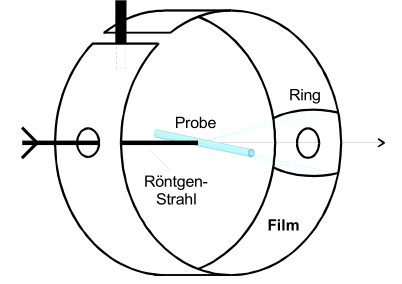
\includegraphics{Aufbau.PNG}
  \caption{Schematischer Aufbau des Versuches.\cite{sample}}
  \label{fig:aufbau}
 \end{figure}
\FloatBarrier
\subsection{Durchführung}
\label{subsec:durch}
Nach der Einstrahlungszeit, die für die Metallprobe $\SI{2}{\hour}$ und für Salzprobe $\SI{4}{\hour}$ beträgt, wird der Filmstreifen unter Rotlicht
aus dem Zylinder entnommen und entwickelt.
Dabei wird wie folgt vorgegangen.
Zu Beginn wird der Film im Entwickler $\SI{15}{\minute}$ geschwenkt,
danach unter Wasser $\SI{1}{\minute}$ abgespült.
Nachdem der Film $\SI{1}{\minute}$ im Unterbrecher gebadet wird, wird
der Film wieder $\SI{1}{\minute}$ unter Wasser abgespült.
Final wird der Film $\SI{5}{\minute}$ im Fixierer geschwenkt und
$5$-$\SI{10}{\minute}$ in Wasser gebadet.
Danch wird der Film $\SI{30}{\minute}$ im Trockenschrank getrocknet.


\subsection{systematische Fehler}
\label{subsec:systerr}
Bei der Messung des Winkels $\theta$
treten durch den Aufbau bedingte zwei systematische Fehler auf.
Zu einem wird der $\theta$-Winkel grundsätzlich zu groß gemessen.
Durch überwiegende Absorption von Röntgenstrahlung in der Probe
findet die Beugung an der Oberfläche des
Probezylinders statt. In Abbildung \ref{fig:error1} wird
der Fehler grafisch dargestellt und nach Bradley und Jay
ergibt sich für die Korrektur
$\Delta \mathrm{a}_{\mathrm{A}}$
zu Gitterkonstante $\mathrm{a}$
\begin{align}
  \frac{\Delta \mathrm{a}_{\mathrm{A}}}{\mathrm{a}}=\frac{\rho}{2\mathrm{R}}\left(1-\frac{\mathrm{R}}{\mathrm{F}}\right)\frac{\cos^2\theta}{\theta}. \label{eqn:sys1}
\end{align}
Dabei entspricht $\rho$ dem Radius der Probe, $R$ dem Kameraradius
und $F$ dem Abstand Fokus-Probe.

\begin{figure}[hhh]
  \centering
  \begin{subfigure}{.49\textwidth}
    \centering
    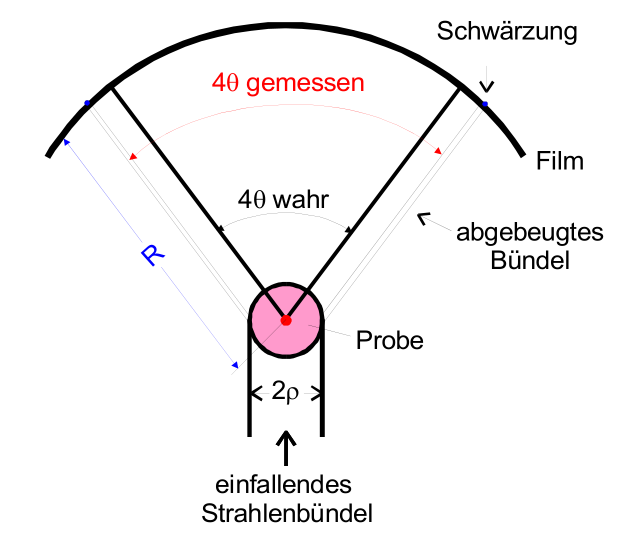
\includegraphics[width=1\textwidth]{Syst_error_1.PNG}
    \caption{Systematischer Fehler bei der Messung von $\theta$ durch
    Absorption an der Oberfläche der Probe.\cite{sample}}
    \label{fig:error1}
  \end{subfigure}
  \begin{subfigure}{.49\textwidth}
    \centering
    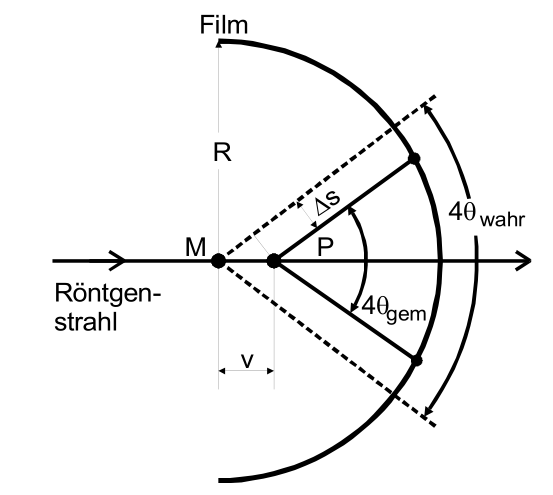
\includegraphics[width=1\textwidth]{Syst_error_2.PNG}
    \caption{Systematischer Fehler bei
    der Messung von $\theta$, da die Probenachse $P$
     und Filmstreifenachse $M$ nicht übereinander liegen.\cite{sample}}
    \label{fig:error2}
  \end{subfigure}
\end{figure}


 % \begin{figure}
 %   \centering
 %   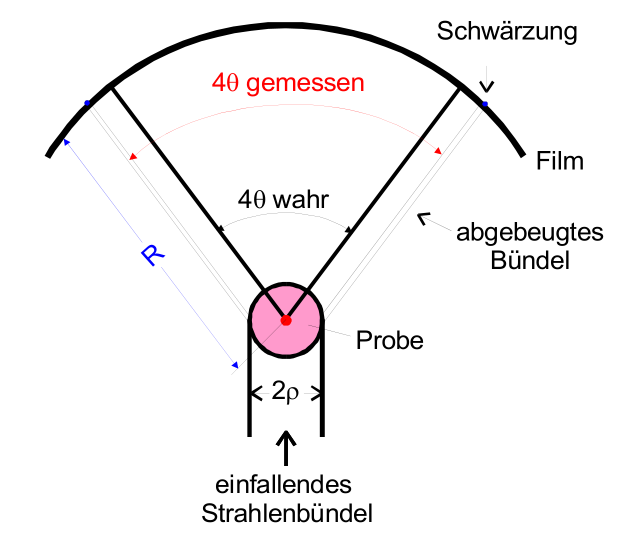
\includegraphics[width=0.5\textwidth]{Syst_error_1.PNG}
 %   \caption{Systematischer Fehler bei der Messung von $\theta$ durch
 %   Absorption an der Oberfläche der Probe.}
 %   \label{fig:error1}
 %  \end{figure}

Zum andern fallen die Zylinderachsen von Probe und Filmstreifen
nur bedingt ineinander, wie in Abbildung \ref{fig:error2} dargestellt .

% \begin{figure}
%   \centering
%   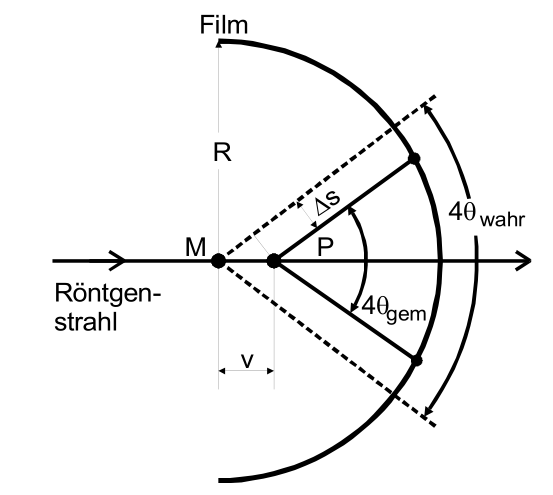
\includegraphics[width=0.5\textwidth]{Syst_error_2.PNG}
%   \caption{Systematischer Fehler bei
%   der Messung von $\theta$, da die Probenachse $P$
%    und Filmstreifenachse $M$ nicht übereinander liegen.}
%   \label{fig:error2}
% \end{figure}
Der Abstand $v$ der zwei Zylinderachsen in der Röntgenstrahl-Ebene
verändert somit den gemessenen Winkel $\theta$.
Für die Korrektur $\Delta a_{\mathrm{V}}$ an der Gitterkonstante $\mathrm{a}$
aus diesem systematischen Fehler ergibt sich somit
\begin{align}
  \frac{\Delta a_{\mathrm{V}}}{\mathrm{a}}=\frac{\mathrm{v}}{\mathrm{R}} \cos^2 \theta. \label{eqn:sys2}
\end{align}
